Dříve \orig{64} než přikročíme k odvození vzorců pro řešení
vyrovnávacích úloh typu IC a CU, srovnáme nejprve ortogonalizaci
matice
%
\begin{align*}
  \tag{7.1}
  A = \vcenter{\hbox{
  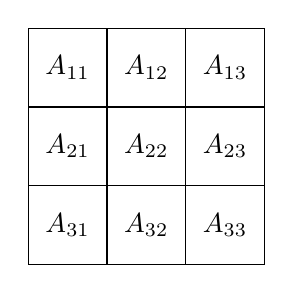
\begin{tikzpicture}[x=1cm,y=1cm]
    \draw (0,2) rectangle (1,3); \draw(0.5,2.5) node{$A_{11}$};
    \draw (1,2) rectangle (2,3); \draw(1.5,2.5) node{$A_{12}$};
    \draw (2,2) rectangle (3,3); \draw(2.5,2.5) node{$A_{13}$};
    \draw (0,1) rectangle (1,2); \draw(0.5,1.5) node{$A_{21}$};
    \draw (1,1) rectangle (2,2); \draw(1.5,1.5) node{$A_{22}$};
    \draw (2,1) rectangle (3,2); \draw(2.5,1.5) node{$A_{23}$};
    \draw (0,0) rectangle (1,1); \draw(0.5,0.5) node{$A_{31}$};
    \draw (1,0) rectangle (2,1); \draw(1.5,0.5) node{$A_{32}$};
    \draw (2,0) rectangle (3,1); \draw(2.5,0.5) node{$A_{33}$};
  \end{tikzpicture} }} \Punc{,}
\end{align*}
%
algoritmem ORTON se zobecněnou ortogonalizací matice
%
\begin{align*}
  \tag{7.2}
  \hspace*{4ex}\vcenter{\hbox{
    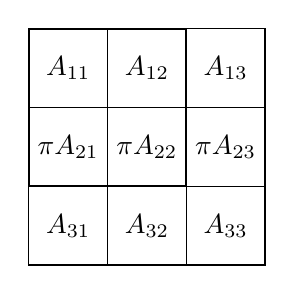
\begin{tikzpicture}[x=1cm,y=1cm]
    \draw[thick] (0,1) rectangle (2,3);
    \draw (0,2) rectangle (1,3); \draw(0.5,2.5) node{$A_{11}$};
    \draw (1,2) rectangle (2,3); \draw(1.5,2.5) node{$A_{12}$};
    \draw (2,2) rectangle (3,3); \draw(2.5,2.5) node{$A_{13}$};
    \draw (0,1) rectangle (1,2); \draw(0.5,1.5) node{$\pi A_{21}$};
    \draw (1,1) rectangle (2,2); \draw(1.5,1.5) node{$\pi A_{22}$};
    \draw (2,1) rectangle (3,2); \draw(2.5,1.5) node{$\pi A_{23}$};
    \draw (0,0) rectangle (1,1); \draw(0.5,0.5) node{$A_{31}$};
    \draw (1,0) rectangle (2,1); \draw(1.5,0.5) node{$A_{32}$};
    \draw (2,0) rectangle (3,1); \draw(2.5,0.5) node{$A_{33}$};
  \end{tikzpicture} }} \Punc{,}
\end{align*}
%
kde $\pi$ je konstanta stejného významu jako ve (5.10). Matici
získanou v prvním případě označme \Wmat.  Výsledkem zpracování matice
(7.2) bude matice $W^{(\pi)}$ v závislosti na volbě konstanty
$\pi$. Lze dokázat, že platí
%
\begin{align*}
  \tag{7.3}
  \begin{array}{lll}
    W_{11} = \lim \,\pi\, W^{(\pi)}_{11} \Punc{,} &
    W_{12} = \lim \,\pi\, W^{(\pi)}_{12} \Punc{,} &
    W_{13} = \lim \,\pi\, W^{(\pi)}_{13} \Punc{,} \\
    W_{21} = \lim \,\pi\, W^{(\pi)}_{21} \Punc{,} &
    W_{22} = \lim \,\pi\, W^{(\pi)}_{22} \Punc{,} &
    W_{23} = \lim \,\pi\, W^{(\pi)}_{23} \Punc{,} \\
    W_{31} = \lim \,\pi\, W^{(\pi)}_{31} \Punc{,} &
    W_{32} = \lim \,\pi\, W^{(\pi)}_{32} \Punc{,} &
    W_{33} = \lim \,\pi\, W^{(\pi)}_{33} \Punc{,} \\[1ex]
    \multicolumn{3}{l}{
    \lim \,\pi\, W^{(\pi)}_{11} =
    \lim \,\pi\, W^{(\pi)}_{22} =
    \lim \,\pi\, W^{(\pi)}_{23} =
    \lim \,\pi\, W^{(\pi)}_{31} = 0 \Punc{,}} \\
  \end{array}
\end{align*}
%
přičemž všechny limity se uvažují pro $\pi \rightarrow \infty$.



\section{Vyrovnání zprostředkujících pozorování s podmínkami}

V kap. 5 \orig{65} jsme ukázali, že úlohy typu IC lze interpretovat
jako zvláštní případ vyrovnání zprostředkujících pozorování, kde váha
jedné skupiny rovnic oprav roste nade všechny meze.  Uvažujme
vyrovnání zprostředkujících pozorování se dvěma skupinami rovnic oprav
%
\begin{align*}
  \tag{7.4}
  \begin{bmatrix}
    v_1 \\ v_2
  \end{bmatrix}^{(\pi)} =
  \begin{bmatrix}
    A_1 & A_2 \\ B_1 & B_2
  \end{bmatrix} x^{(\pi)} +
  \begin{bmatrix}
    l_1 \\ l_2
  \end{bmatrix} \Punc{,}
\end{align*}
%
jejichž váhy jsou dány maticemi $P$ a $\pi^2E$. Vertikální členění
matice soustavy (7.4) je provedeno tak, aby matice $B_1$, byla
čtvercová. Předpokládáme rovněž, že $B_1$ je regulární. V limitě $\pi
\rightarrow \infty$ přejde řešení této úlohy na řešení úlohy typu IC
(s vahami P)
\begin{align*}
  \tag{7.5}
  \begin{bmatrix}
    v \\ 0
  \end{bmatrix} =
  \begin{bmatrix}
    A_1 & A_2 \\ B_1 & B_2
  \end{bmatrix} x +
  \begin{bmatrix}
    l_1 \\ l_2
  \end{bmatrix}
\end{align*}
%
v souladu s (5.1) a (5.2). Jak bylo dokázáno v odst. 3.1,
můžeme úlohu (7.4) řešit zobecněnou ortogonalizací podle schematu
%
\begin{align*}
  \tag{7.6}
  \vcenter{\hbox{
      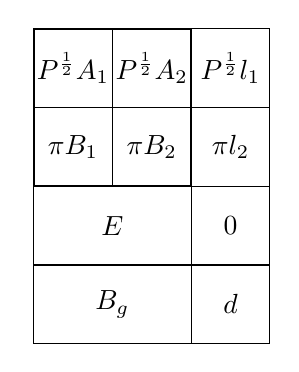
\begin{tikzpicture}[x=1cm,y=1cm]
    \draw [thick] (0,2) rectangle (2,4);
    \draw (0,3) rectangle (1,4); \draw(0.5,3.5) node{$P^{1\over2}A_1$};
    \draw (1,3) rectangle (2,4); \draw(1.5,3.5) node{$P^{1\over2}A_2$};
    \draw (2,3) rectangle (3,4); \draw(2.5,3.5) node{$P^{1\over2}l_1$};
    \draw (0,2) rectangle (1,3); \draw(0.5,2.5) node{$\pi B_1$};
    \draw (1,2) rectangle (2,3); \draw(1.5,2.5) node{$\pi B_2$};
    \draw (2,2) rectangle (3,3); \draw(2.5,2.5) node{$\pi l_2$};
    \draw (0,1) rectangle (2,3); \draw(1.0,1.5) node{$E$};
    \draw (2,1) rectangle (3,2); \draw(2.5,1.5) node{$0$};
    \draw (0,0) rectangle (2,1); \draw(1.0,0.5) node{$B_g$};
    \draw (2,0) rectangle (3,1); \draw(2.5,0.5) node{$d$};
  \end{tikzpicture} }}
  \quad\longrightarrow\quad
  \vcenter{\hbox{
  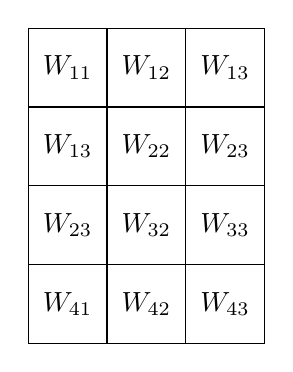
\begin{tikzpicture}[x=1cm,y=1cm]
    \draw (0,3) rectangle (1,4); \draw(0.5,3.5) node{$W_{11}$};
    \draw (1,3) rectangle (2,4); \draw(1.5,3.5) node{$W_{12}$};
    \draw (2,3) rectangle (3,4); \draw(2.5,3.5) node{$W_{13}$};
    \draw (0,2) rectangle (1,3); \draw(0.5,2.5) node{$W_{13}$};
    \draw (1,2) rectangle (2,3); \draw(1.5,2.5) node{$W_{22}$};
    \draw (2,2) rectangle (3,3); \draw(2.5,2.5) node{$W_{23}$};
    \draw (0,1) rectangle (1,2); \draw(0.5,1.5) node{$W_{23}$};
    \draw (1,1) rectangle (2,2); \draw(1.5,1.5) node{$W_{32}$};
    \draw (2,1) rectangle (3,2); \draw(2.5,1.5) node{$W_{33}$};
    \draw (0,0) rectangle (1,1); \draw(0.5,0.5) node{$W_{41}$};
    \draw (1,0) rectangle (2,1); \draw(1.5,0.5) node{$W_{42}$};
    \draw (2,0) rectangle (3,1); \draw(2.5,0.5) node{$W_{43}$};
  \end{tikzpicture} }}^{(\pi)}\hspace{-2ex} \Punc{,}
\end{align*}
%
kde $B_g$ a $d$ odpovídají podle (3.2) funkcím $g$ vyrovnaných
veličin.  Porovnáním matic (7.6) a (3.18) lze potom s využitím vzorců
(3.6) až (3.15) a (3.20) najít řešení úlohy (7.4).
%
%
%
\orig{66}
\begin{align*}
  \tag{7.7}
  x^{(\pi)} &= w_{33}^{(\pi)}, \qquad v_1^{(\pi)} = P^{-{1\over2}} w_{13}^{(\pi)},
  \quad v_2^{(\pi)} = \pi^{-1} w_{23}^{(\pi)},\qquad g^{(\pi)} = w_{43}^{(\pi)},\\
  %
  Q_{LL}^{(\pi)} &=
  \begin{bmatrix}
    P^{-{1\over2}}(W_{11}W_{11}^T + W_{12}W_{12}^T)P^{-{1\over2}} &
    P^{-{1\over2}}(W_{11}W_{21}^T + W_{12}W_{22}^T) \pi^{-1}\\
    \pi^{-1}(W_{21}W_{11}^T + W_{22}W_{12}^T)P^{-{1\over2}} &
    \pi^{-1}(W_{21}W_{21}^T + W_{22}W_{22}^T)\pi^{-1}\\
  \end{bmatrix}^{(\pi)} \Punc{,} \\
  %
  Q_{LX}^{(\pi)} &=
  \begin{bmatrix}
    P^{-{1\over2}}(W_{11}W_{31}^T + W_{12}W_{32}^T)\\
    \pi^{-1}(W_{21}W_{31}^T + W_{22}w_{32}^T) \\
  \end{bmatrix}^{(\pi)} \Punc{,} \\
  %
  Q_{Lg}^{(\pi)} &=
  \begin{bmatrix}
    P^{-{1\over2}}(W_{11}W_{41}^T + W_{12}W_{42}^T)\\
    \pi^{-1}(W_{21}W_{41}^T + W_{22}w_{42}^T) \\
  \end{bmatrix}^{(\pi)} \Punc{,} \\
  %
  Q_{xx}^{(\pi)} &=
  \begin{bmatrix}
    W_{31}W_{31}^T + W_{32}W_{32}^T
  \end{bmatrix}^{(\pi)} \Punc{,} \\
  %
  Q_{xg}^{(\pi)} &=
  \begin{bmatrix}
    W_{31}W_{41}^T + W_{32}W_{42}^T
  \end{bmatrix}^{(\pi)} \Punc{,} \\
  %
  Q_{gg}^{(\pi)} &=
  \begin{bmatrix}
    W_{41}W_{41}^T + W_{42}W_{42}^T
  \end{bmatrix}^{(\pi)} \Punc{.} \\
  %
\end{align*}
%
Přejděme nyní v  (7.7) k limitě $\pi \rightarrow \infty$. Označímě-li
ještě $W = [ W_{ij} ]$ matici získanou ortogonalizací matice $A$
%
\begin{align*}
  \tag{7.8}
  A =
  \vcenter{\hbox{
      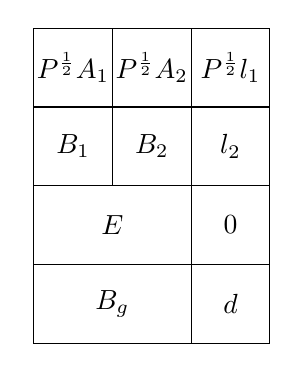
\begin{tikzpicture}[x=1cm,y=1cm]
    %\draw [thick] (0,2) rectangle (2,4);
    \draw (0,3) rectangle (1,4); \draw(0.5,3.5) node{$P^{1\over2}A_1$};
    \draw (1,3) rectangle (2,4); \draw(1.5,3.5) node{$P^{1\over2}A_2$};
    \draw (2,3) rectangle (3,4); \draw(2.5,3.5) node{$P^{1\over2}l_1$};
    \draw (0,2) rectangle (1,3); \draw(0.5,2.5) node{$B_1$};
    \draw (1,2) rectangle (2,3); \draw(1.5,2.5) node{$B_2$};
    \draw (2,2) rectangle (3,3); \draw(2.5,2.5) node{$l_2$};
    \draw (0,1) rectangle (2,3); \draw(1.0,1.5) node{$E$};
    \draw (2,1) rectangle (3,2); \draw(2.5,1.5) node{$0$};
    \draw (0,0) rectangle (2,1); \draw(1.0,0.5) node{$B_g$};
    \draw (2,0) rectangle (3,1); \draw(2.5,0.5) node{$d$};
  \end{tikzpicture} }}
  \quad\longrightarrow\quad
  \vcenter{\hbox{
  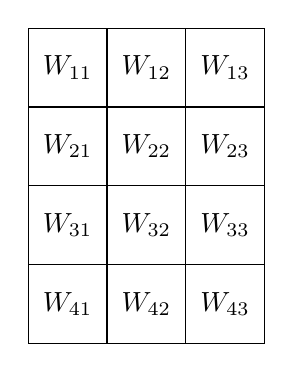
\begin{tikzpicture}[x=1cm,y=1cm]
    \draw (0,3) rectangle (1,4); \draw(0.5,3.5) node{$W_{11}$};
    \draw (1,3) rectangle (2,4); \draw(1.5,3.5) node{$W_{12}$};
    \draw (2,3) rectangle (3,4); \draw(2.5,3.5) node{$W_{13}$};
    \draw (0,2) rectangle (1,3); \draw(0.5,2.5) node{$W_{21}$};
    \draw (1,2) rectangle (2,3); \draw(1.5,2.5) node{$W_{22}$};
    \draw (2,2) rectangle (3,3); \draw(2.5,2.5) node{$W_{23}$};
    \draw (0,1) rectangle (1,2); \draw(0.5,1.5) node{$W_{31}$};
    \draw (1,1) rectangle (2,2); \draw(1.5,1.5) node{$W_{32}$};
    \draw (2,1) rectangle (3,2); \draw(2.5,1.5) node{$W_{33}$};
    \draw (0,0) rectangle (1,1); \draw(0.5,0.5) node{$W_{41}$};
    \draw (1,0) rectangle (2,1); \draw(1.5,0.5) node{$W_{42}$};
    \draw (2,0) rectangle (3,1); \draw(2.5,0.5) node{$W_{43}$};
  \end{tikzpicture} }}^{(\pi)}\hspace{-2ex} = W
\end{align*}
%
algoritmem ORTON, pak s uvážením (7.3) dostaneme po
jednoduchém odvození vzorce řešící úlohu (7.5)
%
%\begin{align*}
%  \tag{7.9}
%  \begin{array}{lll}
%    v = lim_{\pi \rightarrow \infty} P^{-{1\over2}}w_{13}^{(\pi)}
%    = P^{-{1\over2}}w_{12}, &  x = w_{33}, & g = w_{43}, \\
%    Q_{LL} = P^{-{1\over2}}W_{12}W_{12}^TP^{-{1\over2}}, &
%    QLx = P^{-{1\over2}}W_{12}W_{32,} & Q_{Lg} = P^{-{1\over2}}W_{12}W_{42}^T,\\
%    & Q_{xx} = W_{32}W_{32}^T,   &   Q_{xg} = W_{32}W_{42}^T, \\
%    &   &   Q_{qq} = W_{42}W_{42}^T .
%  \end{array}
%\end{align*}
%
\orig{67}
\begin{align*}
  \tag{7.9}
    v &= lim_{\pi \rightarrow \infty} P^{-{1\over2}}w_{13}^{(\pi)}
    = P^{-{1\over2}}w_{12}, &  x &= w_{33}, & g &= w_{43}, \\
    Q_{LL} &= P^{-{1\over2}}W_{12}W_{12}^TP^{-{1\over2}}, &
    QLx &= P^{-{1\over2}}W_{12}W_{32,} & Q_{Lg} &= P^{-{1\over2}}W_{12}W_{42}^T,\\
    && Q_{xx} &= W_{32}W_{32}^T,   &   Q_{xg} &= W_{32}W_{42}^T, \\
    &&&&   Q_{qq} &= W_{42}W_{42}^T .
\end{align*}
%
Ve vzorcích (7.9) nevystupují mj. submatice $W_{22}$ $W_{23}$.  V
důsledku toho můžeme při řešení úloh typu IC algoritmem ORTON vypustit
jeho třetí a případně i druhý krok.  Dále je zřejmé blízká příbuznost
vzorců (7.9) a postupu určení stejných objektů při vyrovnání
zprostředkující pozorování, formulovaného v závěru odst. 3.1. Tato
příbuznost je zákonitá. Mohli bychom totiž dokázat, že v prvním kroku
ORTONu s využitím podmínek mezi neznámými v podstatě modifikujeme
soustavu rovnic oprav eliminací skupiny neznámých a takto
modifikovenou soustavu řešíme zobecněnou ortogonalizací v kroku
čtvrtém.


Podobně jako při vyrovnání zprostředkujících pozorování lze i při
řešení úloh typu IC algoritmem ORTON najít další veličiny,
např. hodnoty obecných funkcí $g = A_g v + B_gx + d$ a
korespondujících váhových koeficientů. V analogii k postupům popsaným
v odst.  3.3.1 stačí v takovém případě buď převést obecné funkce na
speciální tvar (3.2) nebo doplnit matici $A$ v (7.8) maticí $\dot
A^T_g = P^{-{1\over2}} A^T_g $ a ortogonalizovat ji podle schematu

\begin{align*}
  \tag{7.10}
  A =
  \vcenter{\hbox{
      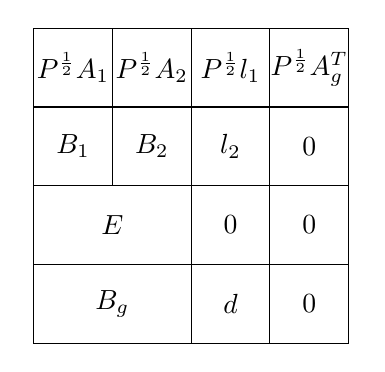
\begin{tikzpicture}[x=1cm,y=1cm]
    %\draw [thick] (0,2) rectangle (2,4);
    \draw (0,3) rectangle (1,4); \draw(0.5,3.5) node{$P^{1\over2}A_1$};
    \draw (1,3) rectangle (2,4); \draw(1.5,3.5) node{$P^{1\over2}A_2$};
    \draw (2,3) rectangle (3,4); \draw(2.5,3.5) node{$P^{1\over2}l_1$};
    \draw (3,3) rectangle (4,4); \draw(3.5,3.5) node{$P^{1\over2}A_g^T$};
    %
    \draw (0,2) rectangle (1,3); \draw(0.5,2.5) node{$B_1$};
    \draw (1,2) rectangle (2,3); \draw(1.5,2.5) node{$B_2$};
    \draw (2,2) rectangle (3,3); \draw(2.5,2.5) node{$l_2$};
    \draw (3,2) rectangle (4,3); \draw(3.5,2.5) node{$0$};
    %
    \draw (0,1) rectangle (2,3); \draw(1.0,1.5) node{$E$};
    \draw (2,1) rectangle (3,2); \draw(2.5,1.5) node{$0$};
    \draw (3,1) rectangle (4,2); \draw(3.5,1.5) node{$0$};
    %
    \draw (0,0) rectangle (2,1); \draw(1.0,0.5) node{$B_g$};
    \draw (2,0) rectangle (3,1); \draw(2.5,0.5) node{$d$};
    \draw (3,0) rectangle (4,1); \draw(3.5,0.5) node{$0$};
  \end{tikzpicture} }}
  \quad\longrightarrow\quad
  \vcenter{\hbox{
  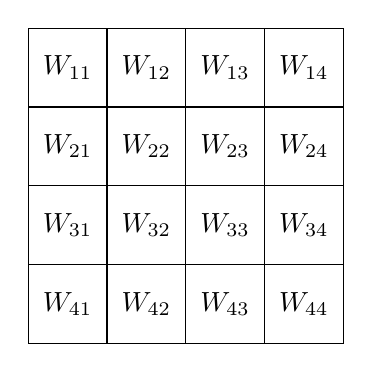
\begin{tikzpicture}[x=1cm,y=1cm]
    \draw (0,3) rectangle (1,4); \draw(0.5,3.5) node{$W_{11}$};
    \draw (1,3) rectangle (2,4); \draw(1.5,3.5) node{$W_{12}$};
    \draw (2,3) rectangle (3,4); \draw(2.5,3.5) node{$W_{13}$};
    \draw (3,3) rectangle (4,4); \draw(3.5,3.5) node{$W_{14}$};
    %
    \draw (0,2) rectangle (1,3); \draw(0.5,2.5) node{$W_{21}$};
    \draw (1,2) rectangle (2,3); \draw(1.5,2.5) node{$W_{22}$};
    \draw (2,2) rectangle (3,3); \draw(2.5,2.5) node{$W_{23}$};
    \draw (3,2) rectangle (4,4); \draw(3.5,2.5) node{$W_{24}$};
    %
    \draw (0,1) rectangle (1,2); \draw(0.5,1.5) node{$W_{31}$};
    \draw (1,1) rectangle (2,2); \draw(1.5,1.5) node{$W_{32}$};
    \draw (2,1) rectangle (3,2); \draw(2.5,1.5) node{$W_{33}$};
    \draw (3,1) rectangle (4,2); \draw(3.5,1.5) node{$W_{34}$};
    %
    \draw (0,0) rectangle (1,1); \draw(0.5,0.5) node{$W_{41}$};
    \draw (1,0) rectangle (2,1); \draw(1.5,0.5) node{$W_{42}$};
    \draw (2,0) rectangle (3,1); \draw(2.5,0.5) node{$W_{43}$};
    \draw (3,0) rectangle (4,1); \draw(3.5,0.5) node{$W_{44}$};
  \end{tikzpicture} }} & \hspace{0.4ex}= W \Punc{.}
\end{align*}
%
%
%
S užitím \orig{68} vzorců (3.43) až (3.46) se potom dá dokázat, že v
limitě $\pi \rightarrow \infty$ platí
%
\begin{align*}
  \tag{7.11}  g     &= W_{43} + W_{14}^TW_{13}\\
  \tag{7.12}  Q_{Lg} &= P^{-{1\over2}} (W_{12}W_{42}^T + \dot A_g^T - W_{14})\\
  \tag{7.13}  Q_{xg} &= W_{32}W_{42}^T - W_{34}\\
  \tag{7.14}  Q_{gg} &= W_{42} W_{42}^T - (W_{44} + W_{44}^T) +
                       (\dot A_g - W_{14}^T)(\dot A_g - W_{14}^T)^T \Punc{.}
\end{align*}


Matici $Q_{gg}'$ váhových koeficientů funkcí v obecném tvaru
%
\begin{align*}
  \tag{7.15}
  g' = A'_gv + B'_gx + C'_gg + d'
\end{align*}
%
lze najít i v těch případech, kdy odpovídající matice v (7.15)
nebyly včleněny do ortogonalizované matice $A$. V korespondenci
se (3.49) a (3.50) platí
%
\begin{align*}
  Q'_{gg} =
  \begin{bmatrix}
    \dot A'_g B'_g C'_g
  \end{bmatrix}
  \begin{bmatrix}
    W_{12}W_{12}^T  &  W_{12}W_{23}^T  &  W_{12}W_{42}^T \\
    W_{32}W_{12}^T  &  W_{32}W_{32}^T  &  W_{32}W_{42}^T \\
    W_{42}W_{12}^T  &  W_{42}W_{32}^T  &  W_{42}W_{42}^T \\
  \end{bmatrix}
  \begin{bmatrix}
    \dot A'_g B'_g C'_g
  \end{bmatrix} ^T
\end{align*}
%
nebo alternativně
%
\begin{align*}
  \tag{7.17}
  Q'_{gg} = (\dot A'_gW_{12} + B'_gW_{32} + C'_gW_{42})
           (\dot A'_gW_{12} + B'_gW_{32} + C'_gW_{42})^T \Punc{.}
\end{align*}
%
V obou posledních vzorcích je kladeno $\dot A'_g = A'_gP^{-{1\over2}}$.



\section{Vyrovnání podmínkových pozorování s neznámými}

Podmínkové rovnice (5.3) zapišme ve tvaru

\begin{align*}
  \tag{7.18}
  \begin{bmatrix}
    A_1^T \\ A_2^T
  \end{bmatrix} v +
  \begin{bmatrix}
    B_1^T \\ B_2^T
  \end{bmatrix} x +
  \begin{bmatrix}
    u_1^T \\ u_2^T
  \end{bmatrix} = 0 \Punc{,}
\end{align*}

\noindent
kde horizontální členění blokových matic je provedeno tak, aby matice
$B_1^T$ byla čtvercová. Kromě toho předpokládejme takové uspořádání
podmínkových rovnic, které zajišťuje regularitu matice $B_1^T$.
Diagonální matici vah označme $P$. Současně s vyrovnáním budeme hledat
funkce vyrovnaných veličin ve tvaru
%
\orig{69}
%
\begin{align*}
  \tag{7.19}
  g^T = A_g^Tv + B_g^T x + d^T
\end{align*}
%
a odpovídající váhové koeficienty.


Předpokládejme nyní, že jsme užili algoritmu ORTON k
ortogonalizaci podle schematu

  \begin{align*}
    \tag{7.20}
    A =
    \vcenter{\hbox{
      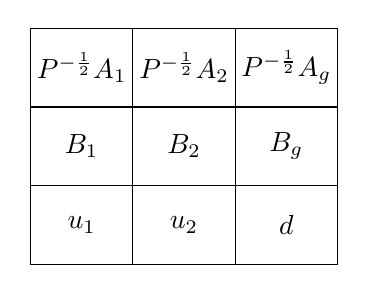
\begin{tikzpicture}[x=1.3cm,y=1cm]
    \draw (0,2) rectangle (1,3); \draw(0.5,2.5) node{$P^{-{1\over2}}A_1$};
    \draw (1,2) rectangle (2,3); \draw(1.5,2.5) node{$P^{-{1\over2}}A_2$};
    \draw (2,2) rectangle (3,3); \draw(2.5,2.5) node{$P^{-{1\over2}}A_g$};
    %
    \draw (0,1) rectangle (1,2); \draw(0.5,1.5) node{$B_1$};
    \draw (1,1) rectangle (2,2); \draw(1.5,1.5) node{$B_2$};
    \draw (2,1) rectangle (3,2); \draw(2.5,1.5) node{$B_g$};
    %
    \draw (0,0) rectangle (1,1); \draw(0.5,0.5) node{$u_1$};
    \draw (1,0) rectangle (2,1); \draw(1.5,0.5) node{$u_2$};
    \draw (2,0) rectangle (3,1); \draw(2.5,0.5) node{$d$};
    \end{tikzpicture} }}
    \quad\longrightarrow\quad
    \vcenter{\hbox{
      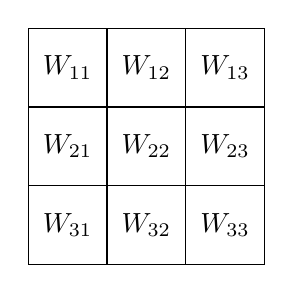
\begin{tikzpicture}[x=1cm,y=1cm]
      \draw (0,2) rectangle (1,3); \draw(0.5,2.5) node{$W_{11}$};
      \draw (1,2) rectangle (2,3); \draw(1.5,2.5) node{$W_{12}$};
      \draw (2,2) rectangle (3,3); \draw(2.5,2.5) node{$W_{13}$};
      \draw (0,1) rectangle (1,2); \draw(0.5,1.5) node{$W_{21}$};
      \draw (1,1) rectangle (2,2); \draw(1.5,1.5) node{$W_{22}$};
      \draw (2,1) rectangle (3,2); \draw(2.5,1.5) node{$W_{23}$};
      \draw (0,0) rectangle (1,1); \draw(0.5,0.5) node{$W_{31}$};
      \draw (1,0) rectangle (2,1); \draw(1.5,0.5) node{$W_{32}$};
      \draw (2,0) rectangle (3,1); \draw(2.5,0.5) node{$W_{33}$};
     \end{tikzpicture} }} \hspace{0.4ex}= W \Punc{.}
  \end{align*}

  \noindent
  Obdobným způsobem jako v odst. 7.1 lze potom dokázat, že platí
  \begin{align*}
    \tag{7.21}
     v &= P^{-{1\over2}}W_{12}w_{32}^T,
    &x &= -(W_{21}w_{31}^T + W_{22}w_{32}^T),
    &g &= w_{33},\\
     Q_{LL} &= P^{-{1\over2}}(E - W_{12}W_{12}^T)P^{-{1\over2}},
    &Q_{Lx} &= P^{-{1\over2}}(W_{11}W_{21}^T + W_{12}W_{22}^T),
    &Q_{Lg} &= P^{-{1\over2}}W_{13},\\
     & & Q_{xx} &= W_{21}W_{11}^TW_{11}W_{21}^T -  W_{22}W_{22}^T,
     &Q_{xg} & = W_{23},\\
     &&&& Q_{gg} &= W_{13}^TW_{13} \Punc{.}
  \end{align*}

  \noindent
  Výpočet matice $Q_{xx}$ podle (7.21) je dosti zdlouhavý. Zpravidla
  vhodnější bude považovat neznámé $x$ za zvláštní případ funkcí
  (7.19) $g_1^T = Ov + E x + 0$ a odpovídající matici zpracovat jako
  čtvrtý blokový sloupec matice $A$ v (7.20) algoritmem ORTON.
  Označíme-li $W_{i4} (i=1,2,3)$ odpovídající submatice matice
  $W$, bude podle (7.21)
%
  \begin{align*}
    \tag{7.22}
    Q_{xx} &= Q_{24}, &Q_{Lx} &= P^{-{1\over2}}, &x &= w_{34}^T \Punc{.}
  \end{align*}
%
  Podobnou úvahu je samozřejmě možné aplikovat nejen na neměřené
  neznámé, ale i na měřené veličiny.
